% Template for ISBI-2018 paper; to be used with:
%          spconf.sty  - ICASSP/ICIP LaTeX style file, and
%          IEEEbib.bst - IEEE bibliography style file.
% --------------------------------------------------------------------------
\documentclass{article}
\usepackage{spconf,amsmath,graphicx}

% Example definitions.
% --------------------
\def\x{{\mathbf x}}
\def\L{{\cal L}}

% Title.
% ------
\title{Scoliosis Screening and Monitoring using Self Contained Ultrasound and Neural Networks}
%
% Single address.
% ---------------
\name{Hastings Greer, Sam Gerber, Marc Niethammer, Roland Kwitt, 
 Matt McCormick, Deepak Chittajallu, Neal Siekierski, Stephen Aylward }
\address{Kitware Inc\\
    Carrboro NC 27510, USA}
%
% For example:
% ------------
%\address{School\\
%	Department\\
%	Address}
%
% Two addresses (uncomment and modify for two-address case).
% ----------------------------------------------------------
%\twoauthors
%  {A. Author-one, B. Author-two\sthanks{Thanks to XYZ agency for funding.}}
%	{School A-B\\
%	Department A-B\\
%	Address A-B}
%  {C. Author-three, D. Author-four\sthanks{The fourth author performed the work
%	while at ...}}
%	{School C-D\\
%	Department C-D\\
%	Address C-D}
%
% More than two addresses
% -----------------------
% \name{Author Name$^{\star \dagger}$ \qquad Author Name$^{\star}$ \qquad Author Name$^{\dagger}$}
%
% \address{$^{\star}$ Affiliation Number One \\
%     $^{\dagger}$}Affiliation Number Two
%
\begin{document}
%\ninept
%
\maketitle
%
\begin{abstract}
We aim to diagnose scoliosis using a self contained ultrasound device that does not require significant training to operate. The device knows its angle relative to vertical using an embedded inertial measurement unit, and it estimates its angle relative to a vertebrae using a neural network analysis of its ultrasound images.  The composition of those angles defines the angle of a vertebrae from vertical.  The maximum difference between vertebrae angles collected from a scan of a spine yields the Cobb angle measure that is used to quantify scoliosis severity. 
\end{abstract}
%
\begin{keywords}
\end{keywords}
%
\section{Introduction}
\label{sec:intro}

Scoliosis is a complex three-dimensional deformity characterized primarily by lateral curvature and rotational deviation of the spine. Different types of scoliosis exist, including congenital, neuromuscular, and syndromic; and the most common is idiopathic, which affects otherwise healthy children. The prevalence of idiopathic scoliosis ranges from 0.5\% to 3\% [Morrissy 2006] with 2-4\% of children ages 6 to 14 having pathologic spinal curves greater than 20°. The most significant risk factor for curve progression is growth, with children entering their adolescent growth spurts at particular risk. While children and adults can live relatively symptom free with small scoliotic curves, as these curves increase in size, the risk of health problems increases concurrently. Surgery is typically recommended for curves over 50 degrees. With curves over 75-80 degrees, significant disability due to restrictive pulmonary and cardiac disease can occur [Haefeli 2006].

Our system is targeting scoliosis screening the general population and quantitatively monitoring scoliosis progression in known cases. As such, our system is intended to be used in the field: at schools, in the offices of general practitioners, and in the offices of pediatric orthopedic surgeons.

\subsection{Screening}
\label{ssec:screen}
Many states in the USA mandate school screening for scoliosis. In general, a scoliometer is used to assess the rotational deformity of a child’s back. Children with scoliometer measurements greater than 5 degrees are referred for further evaluation. X-ray imaging is then typically used. Unfortunately, a scoliometer is quite insensitive and non-specific. It has been reported that the positive predictive value of a scoliometer reading of 5 degrees to detect real scoliosis is only 4\% [Yawn 1999]. This results in a large number of unnecessary referrals to physicians and unneeded X-rays of developing children.

\subsection{Monitoring}
\label{ssec:Monitoring}
 The most common method for monitoring scoliosis is to measure the spinal curvature using Cobb's method [Cobb 1948] from posteroanterior (PA) X-Ray images. A minimum of 10 degrees of Cobb angle is needed to differentiate scoliosis.  However, radiographs are costly and expose children to potentially harmful ionizing radiation. It is estimates that children with scoliosis progression undergo three to seven x-ray images per year, and such radiation exposure increases the risk of leukemia, lung cancer, and breast cancer. [Knott 2014]
 
There has been extensive research into replacing scoliometers and X-Ray imaging with computer-assisted ultrasound imaging systems to reduce costs, increase reliability, and eliminate the need for harmful radiation [Li2010, Chen 2012, Ungi 2014a].  However, most of the ultrasound research systems (1) require the use of external tracking equipment, (2) rely on the operator or an advanced algorithm to precisely locate key landmarks in the ultrasound data, and/or (3) do not provide real-time guidance to the operator, so the operators must still be trained to capture usable scans.  Great progress has been made to tackle each of these challenges, and promising results are being generated ([Chen 2012 and Ungi 2014] have reported ~2° difference compared to radiographs), but we have chosen to explore a self-contained ultrasound-based solution that eliminates the need for external tracking, landmark identification, or extensive operator training.

Our system is based on ultrasound imaging, but an ultrasound image is never presented to the operator.  The operator must be trained regarding how to apply sufficient acoustic gel and how to move the device so as to follow the spine of a child, but the embedded image analysis algorithms and the embedded graphic display provide simple feedback to the operator to ensure that sufficient acoustic gel has been used and that the probe remains over the spine as it is moved.  After a sweep has been completed, the device displays the estimated Cobb angle.

The methods section describes the image analysis and deep learning methods employed by our device.  The experiment section presents results using a spine phantom then indicate that our device can produce results that are more accurate than a scoliometer and nearly as accurate as X-ray imaging.  This paper concludes with a discussion of future steps for device research, development, and validation.

\section{Methods}
\label{sec:methods}

Instead of requiring challenging intermediate steps such as externally tracking an ultrasound probe using optical technologies, reconstructing an ultrasound volume from tracked 2D ultrasound images, determining the coordinates of key landmarks, or registering a volume to an atlas, our system directly estimates the angle between the spine and the ultrasound probe using a neural network. In combination with an internal inertial measurement unit (IMU) to report the angle between the ultrasound probe and vertical, our self-contained, hand-held unit bypasses the traditional intermediate steps and focuses on the measures to be made. The Cobb Angle is defined by the extrema of the estimated angles.

The input training data comes from ultrasound image sequences taken of a model spine immersed in water. The ideal output training data for that input training data is the orientation of the ultrasound probe along each sequence, as measured using an optical tracker.  All training data is accomplished with the model spine straightened, which is sufficient since the neural network only needs to estimate the angle between the ultrasound probe and the underlying vertebrae. The probe is swept up and down the spine while simultaneously rotated along the coronal axis, to obtain 170,000 training images. The ultrasound data is passed to the neural network as B-mode images that have been scaled down to 100x100.

\begin{figure}
\centering
\begin{tabular}{cc}
\centering
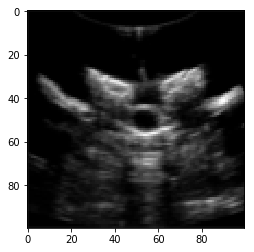
\includegraphics[height=5.5cm,keepaspectratio]{SampleInput}
\end{tabular}
\caption{A sample frame, as passed to the network
}
\end{figure}


Our system’s neural network consists of two parts. A convolutional network modeled after VGG processes each frame, and is trained to predict the angle given a single frame. Then, this network is used to pre-process each frame, and a second fully connected network processes a sliding window of 41 frames by looking at the values of the last layer of the convolutional network.

\begin{table}[ht]
\caption{Convolutional Network}
\begin{tabular}{c c c c}
\hline \\
Type & \# Filters & Stride & Activation \\
\hline
Convolution & 32 & 3x3 & Relu \\
Max Pooling &    & 2x2 &      \\
Convolution & 32 & 3x3 & Relu \\
Max Pooling &    & 2x2 &      \\
Convolution & 32 & 3x3 & Relu \\
Max Pooling &    & 2x2 &      \\
Fully Connected & & 2048 & Relu \\
\end{tabular}
\end{table}

Once the network has been trained, the vertebrae-to-probe angle given by the neural network is subtracted from the probe-to-vertical angle given by the accelerometer embedded in the ultrasound probe. The resulting vertebrae-to-vertical angle sequence is then smoothed with a median filter, and the difference between the maximum and minimum estimated vertebrae-to-vertical angles is the computed Cobb angle.   

\section{Experiment and Results}

As a preliminary validation, we tested our network’s ability to deduce the angle of the ultrasound probe on images of a straight spine acquired while rotating the ultrasound probe as it moved down the spine.  This testing data was captured after (i.e., completely separate from) the training data and consisted of 10,000 images.  See Fig. 2.

\begin{figure}
\centering
\begin{tabular}{cc}
\centering
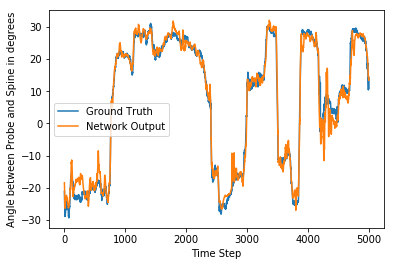
\includegraphics[height=5.5cm,keepaspectratio]{NetworkOutput}
\end{tabular}
\caption{Graph of estimated and actual ultrasound probe angle as it is moved and rotated along a spine.  The neural network can estimate this angle using only the image data.  At transitions between vertebrae and at time step 4300, the angle measures temporarily degrade, but otherwise, the estimated and actual angles are within +/- 2 degrees.  The full system applies median filtering to these data to eliminate local irregularities.
}
\end{figure}
 

To validate the complete system, we manipulated the spine model to depict various Cobb angles / scoliosis severities.   We made physical measurements on the spine to define ground truth.  We then imaged those spines multiple times and used our system to estimate the Cobb angles from those data.  Those results are given in Fig. 3.


Figure 3. 

\section{Automated Operator Guidance}
We anticipate that in order to function with no operator training, our system will need to guide the operator to keep the spinal column visible in the ultrasound image. To that end, we also trained a network with an identical architecture to the single frame network to predict the lateral position of the probe with respect to the spine from the image data. In inference mode this network runs faster than real time, and is sufficiently accurate to provide feedback to the operator such as "Move Right," "Move Left," or "You are Centered." We intend to display this guidance as arrows on the screen of the final product.

\begin{figure}
\centering
\begin{tabular}{cc}
\centering
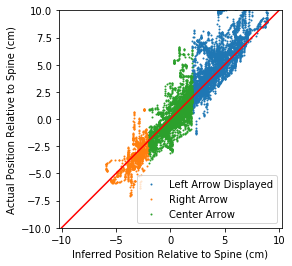
\includegraphics[height=7.5cm,keepaspectratio]{Guidance}
\end{tabular}
\caption{A neural network infers whether the operator needs to move the probe to the left or right to stay centered on the spine
}
\end{figure}

\section{Discussion and Future Work}
We aim to operate this software on our planned hand held, self contained ultrasound device. This device, which runs off of an Intel compute stick and windows 10, will enable an extremely simple and fast workflow, where the operator sweeps the device over the patient’s back, following the onscreen arrows to keep centered on the spine, and then reads the cobb angle off of the screen. Because the device runs the same windows version as the computers we are currently running our research on, we do not anticipate any great difficulty in porting to the new platform


\section{REFERENCES}
\label{sec:ref}

List and number all bibliographical references at the end of the paper.  The references can be numbered in alphabetic order or in order of appearance in the document.  When referring to them in the text, type the corresponding reference number in square brackets as shown at the end of this sentence \cite{C2}.

% References should be produced using the bibtex program from suitable
% BiBTeX files (here: strings, refs, manuals). The IEEEbib.bst bibliography
% style file from IEEE produces unsorted bibliography list.
% -------------------------------------------------------------------------
\bibliographystyle{IEEEbib}
\bibliography{strings,refs}

\end{document}
